\documentclass[10pt,twocolumn,letterpaper]{article}

\usepackage{cvpr}
\usepackage{times}
\usepackage{epsfig}
\usepackage{graphicx}
\usepackage{amsmath}
\usepackage{amssymb}

% Include other packages here, before hyperref.

% If you comment hyperref and then uncomment it, you should delete
% egpaper.aux before re-running latex.  (Or just hit 'q' on the first latex
% run, let it finish, and you should be clear).
\usepackage[breaklinks=true,bookmarks=false]{hyperref}

\cvprfinalcopy % *** Uncomment this line for the final submission

\def\cvprPaperID{****} % *** Enter the CVPR Paper ID here
\def\httilde{\mbox{\tt\raisebox{-.5ex}{\symbol{126}}}}

% Pages are numbered in submission mode, and unnumbered in camera-ready
%\ifcvprfinal\pagestyle{empty}\fi
\setcounter{page}{1}
\begin{document}

%%%%%%%%% TITLE
\title{Object-Centric Latent Video Diffusion Model for High-Quality Video Generation}

\author{Sangyoon Bae\\
Seoul National University\\
{\tt\small stellasybae@snu.ac.kr}
% Uncomment the following lines to add second author
\and
Chanhee Park\\
Seoul National University\\
{\tt\small chan0843@snu.ac.kr}
\and
JinGee Kim\\
Seoul National University\\
{\tt\small jingeekim9@snu.ac.kr}
}

\maketitle
%\thispagestyle{empty}

%%%%%%%%% ABSTRACT
\begin{abstract}
   This assignment is intended to practice your technical paper writing skills. You are about to write three pages of technical paper, excluding extra space for the references. This is a space for the abstract. The abstract is intended to introduce a brief idea of your work and some summary of the experimental results. Now you can guess what texts should be placed in this section: describe a summary of your work, explain why the project is essential, explain what problem you are solving, describe how did you implement, and how it is distinguishable compared to the baseline approaches. The abstract should be concise, so try to make it to be 10 to 15 lines.
\end{abstract}

%%%%%%%%% BODY TEXT
\section{Introduction}

Attention to generative models have peaked as the performance of text and image models are continuing to improve. 
However, generative video models are much more complicated to implement. 
The reason for this is because of the high complexity of high-definition videos and the large computation power needed to run these generative video models.

There have been several previous works on video generation models that include using GANs, VAEs, autoregressive models, and diffusion models.
Among these GAN models have shown promise when generating high-quality images.
However, GAN models suffer from mode collapse and instable training, which makes it difficult to apply GAN models to the more complex video generation problem \cite{brock2018large, karras2019style}.
Other previous works have attempted to use diffusion models to generate high-definition videos \cite{ho2022imagen}.
However, these diffusion models require substantial computational power to generate high-quality videos.
Therefore, latent diffusion models were proposed to solve the high computational cost of generating videos \cite{he2022latent, blattmann2023align}.
Nonetheless, these models can be further improved to produce higher quality and more natural-looking videos.

We propose OLVDM, an object-centric latent video diffusion model that aligns objects during video generation to create natural-looking videos. We modify the original LVDM model and add an object-tracking component to the model. 
When the individual frames are passed through the encoder to the latent space, we use Slot Attention to extract slots from each individual frame. 
Then, we find the correlation between the slots of each frame in the video. 
We add a new component to the loss function that will try and minimize the difference in correlation between each frame. 
Using this method, our model generates more stable videos that surpass previous works in terms of video quality.

We summarize our main contributions as follows:
\begin{itemize}
    \item We propose OLVDM, an object-centric latent video diffusion model that aligns objects during video generation to create natural-looking videos.
    \item OLVDM uses Slot Attention in the latent space to extract object features from each video frame.
    \item A new loss term minimizes the difference in slots between each frame to genereate videos with object-aligned frames.
\end{itemize}

\section{Related work}

\vspace{2mm}
\noindent\textbf{Video Generation Models.}
Video generation has been a prominent area of research with various approaches aiming to capture the complexity and diversity of dynamic scenes. Specifically, latent diffusion models are showing promise in the field of video generation due to the models ability to map the video to a lower-dimensional latent space for efficiency. 
Variational Autoencoders have been extensively explored for video generation tasks \cite{he2018probabilistic}. These models leverage probabilistic latent spaces to capture the underlying structure of the data distribution. However, VAEs often face challenges in generating high-fidelity and temporally coherent videos, limiting their effectiveness in capturing complex dynamics.
Generative Adversarial Networks have shown remarkable success in image generation tasks, leading to their application in video generation \cite{tian2021good}. However, training GANs for video synthesis poses inherent difficulties, including mode collapse and the generation of temporally inconsistent frames.

\vspace{2mm}
\noindent\textbf{Latent Diffusion  Models.}
He~\etal~proposed LVDM, a text-to-video model that processes videos in the latent space to accomplish video generation. 
LVDM uses a 3D autoencoder to map the video frames to a low-dimensional 3D latent space, significantly performing better than previous pixel-space video diffusion models.
They also introduce condition latent perturbation and uncoditional guidance to improve performance when generating longer videos.
However, the results from LVDM suffer from flickering and also cannot focus on the subject of the video effectively.
Blattman~\etal~\cite{blattmann2023align} also proposed a similar latent diffusion model that reshaped the frames of a video to temporally align each individual frame. 
They also use several techniques such as frame interpolation and up-sampling to generate high-definition, high-frame rate videos. 
However, these methods still suffer from mis-alignment between the object and background of the video. 

Previous methods do not sufficiently capture the main subject of a video. In this work, we add a Slot Attention module to extract object-centric representations from each video frame. Then, we add a new loss term to minimize the difference in slots of each frame to generate object-centric videos.
\section{Proposed Method}

We propose a novel video generation method that uses SLOT attention in the latent space to create object-aligned videos. 
We use a similar architecture as LVDM to handle video data in the latent space. 
LVDM uses a lightweight 3D autoencoder that compresses video samples to a lower-dimensional latent space. Then, we use SLOT attention to extract slots from each of the video frames. 
Each slot for each frame holds feature information about each object in the frame. 
Then, the frames go through the diffusion and denoising process to regenerate the original video. 
During the process of generation, we propose a novel correlation loss that minimizes the different between slots for each frame.

\subsection{Video Encoder}
We first describe a lightweight 3D autoencoder used for video compression. 
The input video frames (\(x_0\)) have dimensions \(H \times W \times L \times 3\), where \(H\) is the height, \(W\) is the width, \(L\) is the length (number of frames in the video), and 3 represents the RGB color channels.
The latent representation (\(z_0\)) has dimensions \(h \times w \times l \times c\), where \(h\), \(w\), and \(l\) are spatial dimensions downscaled by factors \(f_s\) (spatial downsampling) and \(f_t\) (temporal downsampling), and \(c\) is the number of channels in the latent space. 
The encoder is responsible for encoding the input video frames (\(x_0\)) into a latent representation (\(z_0\)). The encoder consists of several layers of 3D convolutions, implying that it operates in three dimensions (height, width, and time). 
The decoder reconstructs the video frames (\(\widetilde{x}_0\)) from the encoded latent representation (\(z_0\)). 
Like the encoder, the decoder also comprises several layers of 3D convolutions.

\subsection{Slot Attention}
The described model maintains \(K\) slots, each represented as a vector denoted as \(S_t = [s_{1t}, \ldots, s_{Kt}] \in \mathbb{R}^{K \times D}\), where \(K\) is the number of slots, and \(D\) is the dimensionality of each slot vector.
\section{Results}

It is always great to show something interesting to other people. In this section, you are showing your results. Please put anything you would like to show, such as images, tables, charts, graphs. Remember, just putting results does not end up with a successful paper. What you need to achieve in this section is to provide an \emph{analysis}. If you have excellent results, please describe why it happens. Sometimes, to justify the arguments, an ablation study needs to be performed. For instance, if you have multiple loss functions in your neural network, you produce many results using some of the loss functions intentionally and see the results. In this procedure, you can find what loss function contributes the most to the task.

In this section, you can also compare your results with other methods to justify your arguments. Remember, you had mentioned the pros and cons of the earlier approaches and explained the benefit of the proposed approach in previous sections. By showing comparison with baseline approaches, you can show a \emph{proof} saying that your argument is correct and valid. Remember the arguments regarding the results should be consistent throughout the paper.
\section{Conclusion}

This section describes a quick summary of your work and take-home message from the experiment. Please do not try to reuse texts from abstract because it is redundant. Any discussion for future work would be great instead.

Here is an example. "In this work, we proposed a new algorithm for blabla tasks. The key idea is to introduce blabla to the existing network. Experimental results show that our approach surpasses the prior works. As future work, we are improving blabla part of our pipeline to extend our work to blabla task."
\section{Appendix: \LaTeX\ Tips}

If you want to add a mathematical equations, put the large equation in this way:
\begin{equation}
result = \sum_{i=0}^N \mathcal{F}(e_i, t_i, p_i),
\end{equation}
where $e_i$, $t_i$, $p_i$ stands for the effort, time, and practice for the time stamp $t$, respectively. If you want to add equations in the text, use \$your\_equation\$. The inline equation shall be look like $\sum_i \alpha$. If you are interested in available characters and fonts in Latex, please refer to the nice materials from OverLeaf~\footnote{\url{https://www.overleaf.com/learn/latex/List_of_Greek_letters_and_math_symbols}}.

To put a picture, consider the following examples.
\begin{figure}
    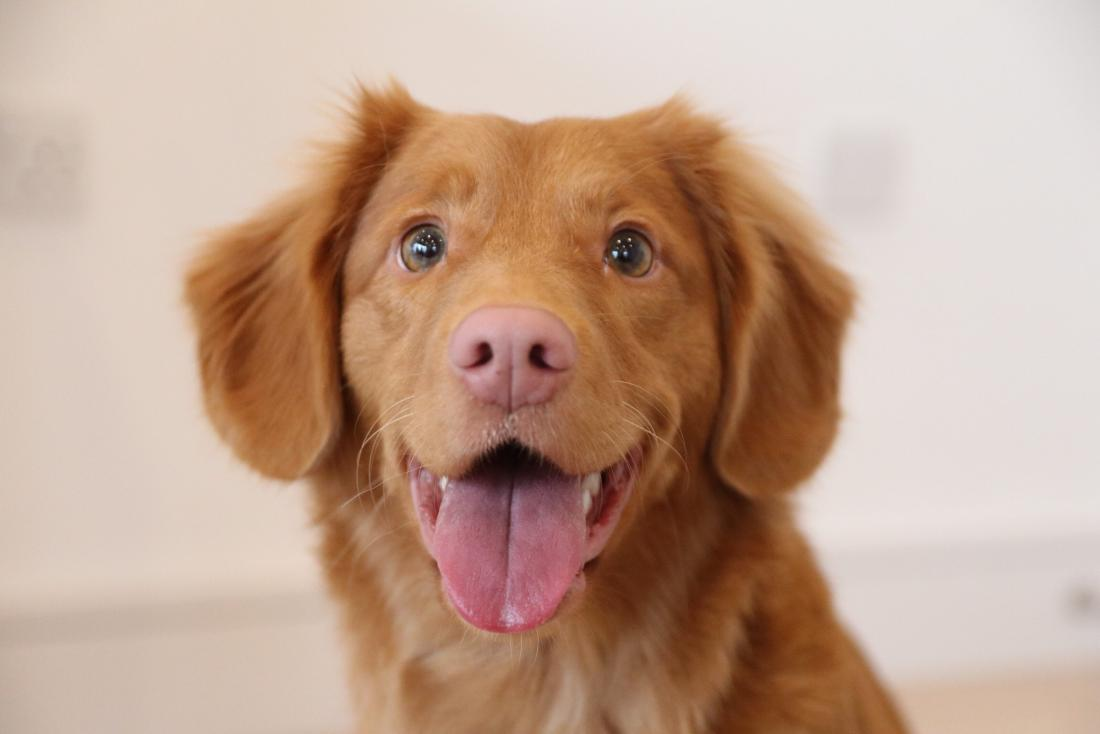
\includegraphics[width=\linewidth]{dog.jpg}
    \caption{You can put a picture and caption in this way. Image taken from Medical News Today.}
\label{fig:dog}
\end{figure}
You can refer the picture in this way. "Fig.~\ref{fig:dog} shows a cute dog. According to Dr. Park, having a pet makes you healthy."
Tou can use the following example to put a table. You can refer "Table.~\ref{table:example} shows a nice results on the xx experiments.."
\begin{table}
\begin{center}
    \begin{tabular}{|l|c|}
    \hline
    Method & Frobnability \\
    \hline\hline
    Theirs & Frumpy \\
    Yours & Frobbly \\
    Ours & Makes one's heart Frob\\
    \hline
    \end{tabular}
\end{center}
\caption{Results.   Ours is better.}
\label{table:example}
\end{table}

To put a comprehensive picture, you can consider any GUI-based image editing software such as photoshop, illustrator, or even PowerPoint. You can export the figure as pdf, jpeg, png. If your picture has some texts, definitely consider using pdf format. Texts in a jpeg and png image will be rasterized, so it will end up losing the beautiful vector graphics.


{\small
\bibliographystyle{ieee_fullname}
\bibliography{egbib}
}

\end{document}
